\section{BGK, AWBS, and Fokker-Planck models in local diffusive regime}
\label{sec:DiffusiveKinetics}

%In a~broad analysis of the~electron transport, any qualitative information
%about its properties are highly welcome. Even better, if one can extract some 
%qualitative information, which provides comparative and reliable results in 
%a~clear way, the~confidence of using a~transport model, 
%e.g. \eqref{eq:AWBS_model}, can lead to efficient yet relatively
%cheap computation cost predictions of real physics.

An~approximate solution to the~\textit{local diffusive regime} 
of electron transport can be found, since it
refers to a~low anisotropy modeled by the~P1 form of EDF  
\begin{equation}
  \tilde{\ft}(z, \vmag, \mu) = \ft^0(z, \vmag) + \mu \ft^1(z, \vmag),
  \label{eq:f_approximation}
\end{equation}
where $z$ is the~spatial coordinate along the~axis $z$, $\vmag$ 
the~magnitude of the~electron velocity. 
%and $\mu = \cos\phi$, where $\phi$ 
%is the~pitch angle with respect to the~axis $z$.

%In the~words of mathematics this corresponds to the~first 
%order expansion in $\mfpei$ and $\mu$ of the~distribution function as
%\begin{equation}
%  \tilde{\ft}(z, \vmag, \mu) = \ft^0(z, \vmag) + \ft^1(z, \vmag) \mfpei\mu ,
%  \label{eq:f_approximation}
%\end{equation}
%where $z$ is the~spatial coordinate along the~axis $z$, $\vmag$ the~magnitude 
%of transport velocity, and 
%$\mfpei = \frac{\vmag}{\nuei} = \frac{\vmag^4}{\Zbar n_e \Gamma}$.
%In other words, one can say that by evaluating numerically $\tilde{\ft}$
%in \eqref{eq:f_approximation}, we accept some error of the~order 
%$O(\mfpei^2) + O(\mu^2)$. The~expansion in a~small parameter $\mfpei$ is also
%coherent with a~time-steady approximation due to the~relation between the~mean
%free path and collision frequency, where the~higher the~collision frequency 
%the~more steady the~solution. 

The~approximate transport solution is then obtained when analyzing 
the~stationary form of \eqref{eq:kinetic_equation} in one spatial dimenstion
(1D) without magnetic field and expressed in spherical coordinates
\begin{equation}
  \mu\left(\pdv{\tilde{f}}{z} 
  + \frac{\qe\Ez}{\me\vmag}\pdv{\tilde{f}}{\vmag}\right) 
  + \frac{\qe\Ez}{\me}\frac{(1-\mu^2)}{\vmag^2}\pdv{\tilde{f}}{\mu}
  %\mu\left(\pdv{f^0}{z} + \frac{\Ez}{\vmag}\pdv{f^0}{\vmag}\right) 
  %+ \frac{\Ez\mfpei}{\vmag^2} f^1 
  = \frac{1}{\vmag}C(\tilde{\ft}) ,
  \label{eq:1D_kinetic_equation}
\end{equation}
where $C$ is a~given collision operator including both e-e and e-i collisions.
Condition of plasma \textit{quasi-neutrality}, 
represented by the~zero current 
$\vect{j} \equiv \qe \int \vect{v} \ft \dI\vect{v} = \vect{0}$ 
in the case of an~unmagnetised plasma in 1D according to \eqref{eq:Ampere}, 
is for the~P1 \eqref{eq:f_approximation} expressed as
\begin{equation}
  \int \vmag f^1 \vmag^2 \dI\vmag = 0 ,
  \label{eq:j0_P1}
\end{equation}
and is accounted for by the~effect of $\Ez$ in \eqref{eq:1D_kinetic_equation}.

The~locality of transport is the~best expressed in terms of the~Knudsen number
$\text{Kn}=\frac{\lambda}{L}$, where $\lambda$ is the~mean free path of electron and
$L$ the~characteristic length scale of plasma. Consequently, plasma conditions
characterized by $text{Kn}\ll1$ correspond to a~local transport regime. 
This measure then
play a~very important role in our analysis, where we use the~electron-electron
and electron-ion mean free paths $\mfpe = \Zbar\mfpei = \frac{\vmag}{\nue}$,
and the~density and temperature plasma scale lengths 
$L_{n_e} = n_e/\pdv{n_e}{z}$ and $L_{T_e} = T_e/\pdv{T_e}{z}$.

In practice, the~Knudsen number of thermal electrons is often used as 
a~measure of the~locality of transport corresponding to given plasma conditions,
where $\text{Kn}(\vth)<0.001$ is considered the~limit of validity of 
the~local transport theory \cite{LMV_1983_7}.


\subsection{BGK local diffusive electron transport}
\label{sec:BGKDiffusiveRegime}

Bhatnagar, Gross, and Krook (BGK) introduced a~very simple form
of a~collision operator \cite{BGK_1954}
\begin{equation}
  C_{BGK}(\tilde{\ft})
  =
  \nue(\fM - \tilde{\ft})
  + \frac{\nuei + \nue}{2}
  \pdv{}{\mu}(1 - \mu^2)\pdv{\tilde{\ft}}{\mu} .
  \label{eq:BGK_model_1D}
\end{equation}
In spite of its~simple form, BGK collision operator \eqref{eq:BGK_model_1D} 
serves as a~useful model providing a~relevant kinetic response, yet only 
qualitative with respect to the~FP collision operator \eqref{eq:LFP_model}.
In particular, the~conservation of kinetic energy, momentum, 
and number of particles is often violated 
\cite{Shkarofsky_Particle_Kinetics_book_1966_24}.

%of the~Boltzmann transport collision 
%operator, because of two reasons: a) it can be treated analytically in 
%the~local diffusive regime; and b) it represents the~so-called phenomenological
%collision operator by explicitly using the~Maxwell-Boltzmann equilibrium 
%distribution $\fM$, which proves to be very useful in coupling of the~nonlocal 
%electron transport to hydrodynamics.

%If one applies the~action of the~right hand side, i.e. of 
%\eqref{eq:BGK_model_1D}, 
%on the~approximation \eqref{eq:f_approximation} and sets the~result to be equal 
%to the~left hand side \eqref{eq:LHS_kinetic_equation}, the~corresponding terms
%in $\mu$ are governed by the~following equations
However, the~form of \eqref{eq:BGK_model_1D} provides a~simple analytical 
treatment of the~local diffusive transport regime, when used in 
\eqref{eq:1D_kinetic_equation}. As a~result, one finds a~simple form of
the~BGK isotropic and anisotropic terms of \eqref{eq:f_approximation} to be
\begin{eqnarray}
  \ft^0 &=& \fM ,
  % \frac{\vth^2}{\vmag^2}f^1 ,
  \label{eq:BGK_f0} \\
  \ft^1 &=& - \frac{\mfpe}{\Zbar + 2}
  \left( \pdv{\fM}{z} + \frac{\qe\Ez}{\me\vmag}\pdv{\fM}{\vmag} \right) ,
  %\left( \pdv{\ft^0}{z} + \frac{\qe\Ez}{\me\vmag}\pdv{\ft^0}{\vmag} \right) , 
  \label{eq:BGK_f1}
\end{eqnarray}
where 
%$Kn = \frac{\mfpe}{L_{n_e}} + \frac{5}{2}\frac{\mfpe}{L_{T_e}}$
a~detailed derivation of \eqref{eq:BGK_f0} and \eqref{eq:BGK_f1} 
can be found in Appendix~\ref{app:DiffusiveKinetics}.
When the~quasi-neutrality constraint \eqref{eq:j0_P1} imposed by $\E_L$
\eqref{app_eq:BGK_Efield} is used, one finally obtains 
the~analytical BGK form of the~anisotropic term %\eqref{eq:f_approximation}
\begin{equation}
  \ft^1 = - \mu 
  \left( \frac{\vmag^2}{2 \vth^2} - 4\right)\frac{1}{\Zbar + 2}
  \frac{\mfpe}{L_{T_e}}\fM
  %\tilde{\ft}_{BGK} = \fM - \mu 
  %\left( \frac{\vmag^2}{2 \vth^2} - 4\right)\frac{1}{\Zbar + 2}
  %\frac{\mfpe}{L_{T_e}}\fM 
  . 
  \label{eq:BGK_approximation}
\end{equation}
The~details about the~BGK distribution function compared to other
collision operators can be found in Section~\ref{sec:SummaryDiffusiveKinetics}.

\subsection{AWBS local diffusive electron transport}
\label{sec:AWBSDiffusiveRegime}
%The~main object of this work presented in Sec~\ref{sec:AWBSmodel} simplifies
%in 1D to a~relatively simple form of the~Boltzmann transport collision operator
%(compared to \eqref{eq:LFP_model})
%\begin{equation}
%  C_{AWBS}(f)
%  = 
%  \vmag \nue^* \pdv{}{\vmag}\left(f - \fM\right) %\\
%  + \frac{\nuei + \nue^*}{2}\pdv{}{\mu}(1 - \mu^2)\pdv{f}{\mu} .
%  \label{eq:AWBS_model_1D}
%\end{equation}
Similarly to the~BGK model, the~AWBS collision operator \ref{eq:AWBS_model} 
explicitly uses equilibration to the~Maxwell-Boltzmann distribution $\fM$. 
On the~other hand, AWBS originates from $C_H$, which is derived from 
the~full FP operator \eqref{eq:LFP_model}. This makes the~AWBS operator 
to be superior to the~BGK operator, which is considered a~purely
phenomenological model.
%and also, 
%makes it a~very attractive model of the~nonlocal electron
%transport to be coupled to hydrodynamics via the~plasma electron temperature 
%and density.

%A~qualitative information about the~AWBS model is obtained while repeating
%the~action on \eqref{eq:f_approximation} by the~left hand side 
%\eqref{eq:LHS_kinetic_equation} and by the~right hand side 
%\eqref{eq:AWBS_model_1D} and setting the~equality. The~corresponding terms
%in $\mu$ are then governed by the~following equations
If \eqref{eq:AWBS_model} is used in \eqref{eq:1D_kinetic_equation}, one obtains
the~following equations governing the~AWBS isotropic and anisotropic terms of 
\eqref{eq:f_approximation}
\begin{eqnarray}
  \pdv{f^0}{\vmag} &=& \pdv{\fM}{\vmag} ,
  %+ Kn \frac{\vth^2}{\vmag^2}\frac{f^1}{\vmag} ,
  \label{eq:AWBS_f0} \\
  \pdv{f^1}{\vmag}  
  - \frac{\Zbar +  r_A}{\vmag r_A} f^1 &=& 
  %\frac{\mfpe}{\vmag\zeta}
  %\left(\pdv{f^0}{z} + \frac{\qe\Ez}{\me\vmag}\pdv{f^0}{\vmag}\right) ,
  \frac{\mfpe}{\vmag r_A}
  \left(\pdv{\fM}{z} + \frac{\qe\Ez}{\me\vmag}\pdv{\fM}{\vmag}\right) ,
  \label{eq:AWBS_f1} 
  %\\  
  %\frac{\vmag}{\Zbar}\pdv{f^1}{\vmag} + \frac{4}{\Zbar}f^1 
  %- \frac{\Zbar + 1}{\Zbar} f^1 &=&
  %\pdv{f^0}{z} + \frac{\tilde{E}_z}{\vmag}\pdv{f^0}{\vmag}
  %\nonumber
\end{eqnarray}
where $ r_A$ represents a~scaling parameter defining the~modified
e-e collision frequency as $\nue^* =  r_A \nue$.
A~detailed derivation of \eqref{eq:AWBS_f0} and \eqref{eq:AWBS_f1} 
can be found in Appendix~\ref{app:DiffusiveKinetics}.
%One observes that $\ft^0$ goes to Maxwellian when 
%the~local regime of transport is settled. 
%Indeed, according to equation~\eqref{eq:AWBS_f0} the~derivative 
%$\pdv{\ft^0}{\vmag}\rightarrow\pdv{\fM}{\vmag}$  when $Kn\ll1$ for any 
%electron velocity, thus leading to $\ft^0\rightarrow\fM$.
Consequently, one finds the~AWBS model equation for $\ft^1$ 
in local diffusive regime to be
%i.e. $\ft^0 = \fM + O(\mfpei^2)$, however, the~$\ft^1$ does not have 
%a~straightforward analytic formula. In reality, $\ft^1$ arises from 
%the~ordinary differential equation 
%(by inserting $\fM$ into \eqref{eq:AWBS_f1})
\begin{multline}
  \pdv{\ft^1}{\vmag} 
  - \frac{\Zbar +  r_A}{\vmag r_A}\ft^1
  = \\
  \frac{\mfpe}{\vmag r_A}\left(\frac{1}{L_{n_e}} + 
  \left( \frac{\vmag^2}{2 \vth^2} - \frac{3}{2}\right)
  \frac{1}{L_{T_e}} - \frac{\qe\Ez}{\me\vth^2}\right)\fM .
  %\frac{\mfpe}{\vmag}\left(\frac{1}{n_e}\pdv{n_e}{z} + 
  %\left( \frac{\vmag^2}{2 \vth^2} - \frac{3}{2}\right)
  %\frac{1}{T}\pdv{T}{z} - \frac{\qe\Ez}{\me\vth^2}\right)\fM .
  \label{eq:AWBS_f1_ODE}
\end{multline}
The~solution of \eqref{eq:AWBS_f1_ODE} can be found in terms of 
upper incomplete gamma function $\tilde{\Gamma}$ 
(see \appref{app:DiffusiveKinetics})
\begin{equation}
  \ft^1_{\text{AWBS}} = - \frac{d}{\vmag^a} 
  \left(b~\tilde{\Gamma}{\left(\frac{a+6}{2}, \frac{\vmag^2}{2\vth^2}\right)}
  + c~\tilde{\Gamma}{\left(\frac{a+4}{2}, \frac{\vmag^2}{2\vth^2}\right)}\right)
  ,
  \label{eq:AWBS_analytic_solution}
\end{equation}
where 
$a = -\frac{\Zbar + r_A}{r_A}$, $b = \frac{1}{L_{\Te}}$, 
$c = \frac{1}{L_{\ed}} - \frac{3}{2}\frac{1}{L_{\Te}} 
- \frac{\qe\Ez}{\me\vth^2}$, and
$d = \frac{2^{\frac{a + 2}{2}} \vth^{a + 1}}{r_A (2\pi)^{\frac{3}{2}} \Gamma}$.
Nevertheless, a~numerical solution of \eqref{eq:AWBS_f1_ODE} needs to be 
adopted for higher $\Zbar$  (see \appref{app:DiffusiveKinetics}).
The~\textit{quasi-neutrality} constraint \eqref{eq:j0_P1} applied to
$\ft^1_{\text{AWBS}}$ leads to $\Ez = \E_L$ \eqref{app_eq:BGK_Efield} 
independently from $\Zbar$ and $r_A$. 

%The~details about the~AWBS distribution function compared to other
%collision operators and a~proper evaluation of the~scaling parameter $r_A$
%can be found in Section~\ref{sec:SummaryDiffusiveKinetics}.

\subsection{Fokker-Planck local diffusive electron transport}
\label{sec:FPDiffusiveRegime}

Solution to the~1D transport equation \eqref{eq:1D_kinetic_equation}
using the~Fokker-Planck collision operator \eqref{eq:LFP_model}
is very ambitious, as demonstrated in 
\cite{Chandrasekhar_RMP1943, CSR_1950, Rosenbluth_PR1957}, fortunately, one 
can use the~explicit evaluation of the~electron distribution function
published in \cite{SpitzerHarm_PR1953}, which takes the~following form
\begin{multline}
  %\ft^1(\vmag, \mu) 
  \ft^1_{\text{SH}} = %\frac{\me^2}{4 \pi \qe^4\lnc} 
  \frac{\vtwoh^4}{\Gamma\Zbar n_e}\\
  \left( 2\tilde{D}_T\left(\frac{\vmag}{\vtwoh}\right) 
  + \frac{3}{2}\frac{\gamma_T}{\gamma_E} 
  \tilde{D}_E\left(\frac{\vmag}{\vtwoh}\right) \right)%\\ 
  \frac{\fM}{T}\pdv{T_e}{z}  ,
  \label{eq:f1_SH}
\end{multline}
where $\tilde{D}_T(x) = \Zbar D_{T}(x) / B$, 
$\tilde{D}_E(x) = \Zbar D_{E}(x) / A$, $\gamma_T$,
and $\gamma_E$ are numerical values in TABLE~I, TABLE~II, and
TABLE~III in \cite{SpitzerHarm_PR1953}, and 
$\vtwoh = \sqrt{\frac{\kB T_e}{2\me}}$.

One should be aware, that the~solution of \eqref{eq:1D_kinetic_equation}
with the~full FP collision operator reveals importance of
e-e Coulomb collisions, which is emphasized in the~$\Zbar$ dependence 
of the~distribution function, current, heat flux, 
electric field according to \eqref{eq:j0_P1}, etc.
In particular, the latter exhibits the~following dependence 
\cite{SpitzerHarm_PR1953}
\begin{equation}
  \E = \frac{\me \vth^2}{\qe}
  \left(\frac{\nabla n_e}{n_e} + 
  \left(1 + \frac{3}{2}\frac{\Zbar + 0.477}{\Zbar + 2.15} \right)
  \frac{\nabla T_e}{T_e} \right),
  \label{eq:SH_Efield} 
\end{equation}
which for $\Zbar\gg1$ corresponds to the~classical Lorentz electric field 
\eqref{app_eq:BGK_Efield}.

%In the~case of high $\Zbar$ limit, $\gamma_T \rightarrow 1$,
%$\gamma_E \rightarrow 1$, $d_E(x) = x^4$, and $d_T(x) = x^4 (2.5 - x^2)/2$
%\cite{SpitzerHarm_PR1953}, which leads to the~standard Lorentz gas model
%\begin{equation}
%   f_1(\vmag, \theta) = \cos(\theta) \frac{\me^2}{4 \pi e^4\lnc} 
%  \frac{\vmag^4}{\Zbar}\left( 4 - \frac{\vmag^2}{\vtwoh^2} \right) 
%  \frac{\fM(\vmag)}{n_e}\frac{\nabla T}{T}  ,
%  \label{eq:f1_Lorentz} 
%\end{equation} 

\subsection{Summary of the~BGK, AWBS, and Fokker-Planck local diffusive 
transport}
\label{sec:SummaryDiffusiveKinetics}

Ever since the~SH paper \cite{SpitzerHarm_PR1953}, the~effect of microscopic
electron transport on the~current $\int \qe \vv \tilde{\ft} \, \dI\vv$ 
and the~heat flux $\int \frac{\me |\vv|^2}{2} \vv \tilde{\ft} \, \dI\vv$ 
in plasmas
under local diffusive conditions has been understood. By overcoming some 
delicate aspects of the~numerical solution to \eqref{eq:LFP_model} presented 
in \cite{CSR_1950}, the~effect of electron-electron collisions
was quantified and dependence on $\Zbar$ of the~heat flux
$\vect{q}$ was approximated as \cite{SpitzerHarm_PR1953, Epperlein_PoFB1991} 
\begin{equation}
  \vect{q} = \xi(\Zbar)~\vect{q}_L 
  = \frac{\Zbar + 0.24}{\Zbar + 4.2} \vect{q}_L ,
  \label{eq:qSH_approximation}
\end{equation}
where 
$\xi$ is the~$\Zbar$-dependence \cite{Epperlein_PoFB1991} approximation and
$\vect{q}_L$
%$\vect{q}_L = \kappa T_e^{\frac{5}{2}}\nabla T_e$ 
is the~heat flux given 
by the~Lorentz gas model \cite{Lorentz_1905} 
\begin{equation}
  \ft^1_{\text{Lorentz}} = - \mu 
  \left( \frac{\vmag^2}{2 \vth^2} - 4\right)
  \frac{\mfpei}{L_{T_e}}\fM
  . 
  \label{eq:Lorentz_approximation}
\end{equation}
 
In the~case of BGK the~collision operator \eqref{eq:BGK_model_1D} needs to be 
corrected in order to provide a~same local behavior as 
\eqref{eq:qSH_approximation}, i.e. a~correct dependence on 
$\Zbar$. Consequently, we define a~scaling formula 
\begin{equation}
  r_B(\Zbar) = \frac{\zeta\Zbar}{\xi(\Zbar + 2 \zeta)} ,
  \label{eq:BGK_r_scaling}
\end{equation}
based on comparison of the~formula \eqref{eq:BGK_approximation} to 
$\xi \ft^1_{\text{Lorentz}}$ and we write a~consistent local diffusion version
of BGK 
\begin{equation}
  C_{BGK}(\tilde{\ft})
  =
  r_B \nue(\fM - \tilde{\ft})
  + \frac{r_B}{\zeta}\frac{\nuei + \zeta\nue}{2}
  \pdv{}{\mu}(1 - \mu^2)\pdv{\tilde{\ft}}{\mu}
  %\nue^{BGK} = \frac{r\nue}{\xi},\quad \nuei^{BGK} = \frac{\nuei}{\xi}
   ,
  \label{eq:BGK_scaling}
\end{equation}
where the~constant $\zeta$ can be set arbitrarily, because it does not affect 
the~local EDF of \eqref{eq:BGK_scaling}
\begin{equation}
  \ft^1_{\text{BGK}} = - \mu 
  \left( \frac{\vmag^2}{2 \vth^2} - 4\right)\frac{\zeta}{r_B(\Zbar)}
  \frac{1}{\Zbar + 2\zeta}\frac{\mfpe}{L_{T_e}}\fM
  ,
  \label{eq:f1BGK_approximation}
\end{equation}
which is identical to $\xi \ft^1_{\text{Lorentz}}$ for any value of $\zeta$.
One should notice that $r_B(\Zbar\gg1) = \zeta$, i.e. $\zeta$ can be adjusted 
appropriately for example to better address the~transport in nonlocal regime.
%\textit{$\zeta = 2$ gives $r_B(\Zbar\gg1) = \zeta$, 
%which makes sence compared to John's hohlraum.}

\begin{table}
\begin{center}
  \begin{tabular}{c|ccccc}
    \hline\hline\\
    %$\Zbar$ & $1$ & $2$ & $4$ & $16$ & $\infty$ \\\\
    & $\,\Zbar=1\,$ & $\,\Zbar=2\,$ & $\,\Zbar=4\,$ & $\,\Zbar=16\,$ & $\,\Zbar=116\,$ \\\\
    \hline\\
    $\bar{\Delta}\vect{q}_{AWBS}$ & 0.057 & 0.004 & 0.037 & 0.021 & 0.004 \\\\
    \hline\\
    $\phi(\Zbar)$ & -0.037 & -0.003 & 0.04 & 0.058 & 0.065 \\\\ 
    \hline\hline
  \end{tabular}
  \caption{
  Relative error $\bar{\Delta}\vect{q}_{AWBS} = 
  |\vect{q}_{AWBS} - \vect{q}_{SH}| / \vect{q}_{SH}$ of 
  the~$\nue^* = \frac{\nue}{2}$~scaling used in the~AWBS model
  \refeq{eq:AWBS_model} showing the~discrepancy 
  (maximum 6$\%$) with respect to the~original solution of 
  the~heat flux given by numerical solution in Spitzer and Harm 
  \cite{SpitzerHarm_PR1953}. The~values of $\phi(\Zbar)$ (a~weak dependence 
  \eqref{eq:qAWBS_approximation}) are also shown. 
  }
\label{tab:qAWBS}
\end{center}
\end{table}

We have performed an~extensive analysis in the case of 
the~AWBS operator in order to obtain the~heat flux behavior while varying 
$\Zbar$. As expected, the~heat flux magnitude did not match exactly 
the~$\Zbar$-dependence \eqref{eq:qSH_approximation}, e.g. for $\Zbar=1$
the~AWBS heat flux was about 60$\%$ less than the~SH calculation, while
there was a~perfect match in the case of $\Zbar\gg1$. By assuming that the~e-e
collisions are responsible for this inadequacy, we searched for a~scaling of
$\nue$ in \eqref{eq:AWBS_model}. Interestingly, we found an~almost constant
scaling $ r_A$, i.e. with a~very weak dependence on $\Zbar$ as  
\begin{equation}
  \nue^* =  r_A(\Zbar)~\nue 
  = \left(\frac{1}{2} + \phi(\Zbar)\right) \nue \approx \frac{\nue}{2} ,
  \label{eq:qAWBS_approximation}
\end{equation}
where can be approximated as 
$\phi(\Zbar) = \frac{0.59 \Zbar - 1.11}{8.37 \Zbar + 5.15} \ll\frac{1}{2}$ 
for any $\Zbar$, i.e. we decide to use $r_A = \frac{1}{2}$.
Indeed, \tabref{tab:qAWBS} shows $\phi(\Zbar)$ and corresponding relative
error (maximum 6$\%$) of the~heat flux modeled by 
\eqref{eq:AWBS_model} vs. SH results represented by 
\eqref{eq:qSH_approximation}. It should be noted that the~error is calculated 
with respect to original values presented in TABLE~III in 
\cite{SpitzerHarm_PR1953}.  
 
The~electron-electron collisions scaling 
\cite{Epperlein_PoFB1991} represented by 
\eqref{eq:qSH_approximation} provides only an~integrated information about
the~heat flux magnitude. If one takes a~closer look at the~distribution
function itself, the~conformity of the~modified AWBS collision operator
is even more emphasized as can be seen in \figref{fig:q1s_summary} showing
the~flux moment in function of the~absolute value of velocity
\begin{equation}
  q_1 = \frac{\me\vmag^2}{2}\vmag \ft^1 \vmag^2 .
  \label{eq:q1}
\end{equation}
In the~case of the~high $\Zbar$ plasma ($\Zbar = 116$), 
AWBS exactly aligns with the~Lorentz gas limit \eqref{eq:Lorentz_approximation}.
In the~opposite case of the~low
$\Zbar$ Hydrogen plasma ($\Zbar = 1$), the~AWBS distribution function 
approaches closely the~numerical SH solution \eqref{eq:f1_SH}. 
BGK \eqref{eq:BGK_scaling} takes 
the~Lorentz gas distribution function for any $\Zbar$ 
only scaled by $\xi$.  
The~AWBS collision operator \eqref{eq:AWBS_model} (red dashed line) 
%represented by a~derivative with respect to $\vmag$ 
provides 
a~significant improvement with respect to the~SH (Fokker-Planck) solution
\eqref{eq:f1_SH} (solid black line) compared to the~simplest BGK model 
\eqref{eq:f1BGK_approximation} (dashed-dot blue line) 
in \figref{fig:q1s_summary}.

\begin{figure}[tbh]
  \begin{center}
    \begin{tabular}{c}
      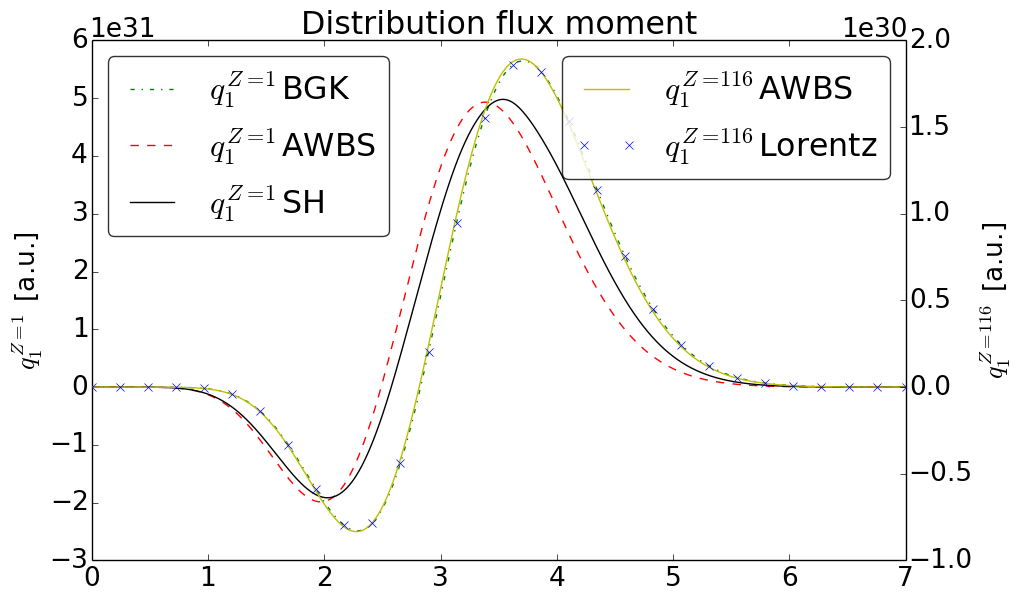
\includegraphics[width=0.5\textwidth]{q1s.png}
    \end{tabular}
  \caption{  
  The~flux velocity moment of the~anisotropic part of the~electron distribution 
  function in low $\Zbar=1$ and high $\Zbar=116$ plasmas in diffusive regime. 
  In the~case of $\Zbar = 1$ the~AWBS model matches very well 
  the~reference solution given by the~SH calculation \cite{SpitzerHarm_PR1953} 
  in comparison to the~BGK model. In the~case of $\Zbar = 116$ the~AWBS model
  aligns exactly with the~Lorentz gas approximation as expected. 
  The~BGK and the~SH curves are not shown for $\Zbar = 116$, but also 
  correspond to the~Lorentz gas distribution function.
  }
  \label{fig:q1s_summary}
  \end{center} 
\end{figure}

%At last, we provide a~quantitative information with respect to the~dominant 
%velocity of electrons contributing to the~heat flux. In the~high $\Zbar$ case
%all the~models give 3.7$\times \vth$, while SH solution gives 3.5$\times \vth$
%and AWBS 3.4$\times \vth$ in the~case of low $\Zbar$ plasmas, thus showing 
%the~right tendency of the~maximum velocity shift modeled by the~modified AWBS
%collision operator \eqref{eq:AWBS_model}.
%\begin{itemize} 
%  \item Point out the~behavior of the~maximum velocity of $q_1$, Lorentz 3.71, SHZ1 3.53, AWBSZ1 3.39.
%\end{itemize}

